\chapter{Case Studies in English Diachrony}\label{ch:diachron}
\section{Introduction}
This chapter applies the analysis presented in the previous three chapters to a large scale case study, namely diachronic development in recipient ditransitive syntax in the history of English. As discussed in the introduction, quantitative (and especially) diachronic studies can provide a useful independent verification of analyses developed on the basis of acceptability judgements. Crucially, data from language production can provide independent verification of theories developed primarily from language comprehension (i.e., acceptability judgements).

The problem of finding empirical validation of theoretical claims is made acute by the nature of the types of claims made in theoretical linguistics. Building on the work starting during the cognitive revolution in the 50s and 60s, the goal of generative linguistics has been to study the linguistic competence of speakers, which consists of the language specific information that is needed to use a language natively \citep{Chomsky.1981,Chomsky.1986}. As will be shown below (in particular when looking at passivisation), this linguistic competence can be separated into grammatical and non-grammatical competences. This distinction between grammatical and non-grammatical competences depends on a specific notion of grammar.

A grammar can be thought of as a list of the possible sound--meaning pairs in a language. Since at least \cite{Chomsky.1965}, it has been recognised that this list is infinitely long for any natural language (because of the recursive nature of natural language). Generative grammar has endevoured to describe rules which are capable of generating the correct sound--meaning pairs. Often, an even simpler goal is attempted, namely to separate strings (chunks of sound) into two sets: (a) the strings that have at least one meaning associated with them (grammatical strings) and (b) the strings that have no meaning associated with them (ungrammatical strings). Note that these meanings do not need to be plausible meanings that any speaker would ever need to use in actual discourse; all that is necessary for a string to be grammatical is that it have \textbf{some} meaning associated with it.\footnote{The classic example from Chomsky's work is ``Colourless green ideas sleep furiously'', which certainly has no real world referents, but is grammatical and has a meaning associated with it (simply a nonsensical meaning). Given that contradictions are stateable in natural languages, whatever our definition of meaning is for grammaticality, it must be able to include nonsensical meanings.}

Given the rampant ambiguity in natural language, the grammar of natural languages often associates multiple strings with a particular meaning (and multiple meanings with a particular string). Since the purpose of the grammar is to simply list whether a string is associated with an utterance, it cannot help a speaker decide which string to use of the strings compatible with the meaning they are trying to express. This problem of knowing which of the options produced by the grammar to use in any particular circumstance is an equally important part of any native speakers linguistic competence. These choices are often impacted by language specific implementations of general social or psychological factors (see \cite{Bresnan.2007,Bresnan.2010,Zeevat.2014} and \cite{Tamminga.2016} for a discussion of these issues and their relationship to the grammar). Unfortunately, it has been known since the beginning of this enterprise that there is no direct evidence of linguistic competence (see \cite{Schutze.1996} for a discussion of early claims about this issue), which is typical of knowledge and psychological constructs. Instead, it has been necessary to deduce the nature of the linguistic knowledge by studying its effects on language performance (see \citealt{Stroud.2012,Phillips.2013, Phillips.2013b, Phillips.2013c} for an arguments that acceptability judgements are fundamentally performative).

One of the most prominent types of linguistic performance to be used in theoretical linguistics is the acceptability judgement. These judgements reflect a native speakers sensation of naturalness/unnaturalness upon encountering a particular linguistic utterance. These sensations have a cognitive reality similar to that of pain sensations \citep{Schutze.2014}. A major advantage to the acceptability judgement is that even utterances that would never occur in natural production (due to the combination of factors each of which is extremely infrequent) can still be studied. However, as mentioned in the first chapter, grammaticality is only one aspect that contributes to the sensation of naturalness; other factors such as pragmatic concerns can often render a perfectly grammatical utterance unnatural (e.g., because there is a more concise grammatical way of conveying the same information). Trained linguists (and ideal native language informants) are able to minimise contextual factors that impact naturalness by attempting to evaluate the utterance in a number of hypothetical linguistic contexts, but these techniques cannot rescue a grammatical utterance that is ruled out because of universal, overwhelming problems. These non-grammatical problems often have a gradual impact on acceptability, reflect a gradient notion of pragmatic infelicity or psychological complexity \citep{Bresnan.2007,Bresnan.2010,Schutze.2014}.

Quantitative studies of language performance is useful for isolating these gradient factors, so that they can be factored out when studying grammaticality using performance data. Since corpora (ideally) provide multiple instances of the relevant features in a variety of pragmatic contexts, the gradient effects of non-grammatical factors can be investigated for the observed contexts and statistically extrapolated to unobserved contexts. In addition, corpora provide a means of studying diachronic processes that cannot be studied using traditional acceptability judgements, since the earlier speakers in the diachronic process are unavailable for consultation. Assuming that language change cannot radically alter the underlying grammar (since the speakers of the new variety must participate in a speech community with speakers of the old variety), it is possible to provide independent evidence of the internal structure of the relevant grammatical processes.

This chapter will begin by reviewing the analyses from the previous three chapters and discussing the diachronic implication of these analyses. This will be followed by looking at two independent changes in the history of English. The first change is the change in recipient marking, ranging from synthetic dative case in Old English to the current distribution of `to' in modern American English. Finally, the fall and rise of recipient passivisation will be examined going from Old English to modern American English.

\section{Theoretical Issues}
	Since this dissertation argues that all languages have the same underlying configuration of recipient and theme (i.e., the recipient is introduced as a dative PP in the specifier of an applicative phrase), I predict that there should be no diachronic development in base generation. However, there are a number of transformations that can apply to the base generated order and different stages of the language can vary as to which operations are grammatical and when they should apply.

	One of the major factors that impact the surface realisation of recipients is allomorphy with respect to the morphological realisation of the dative P-head. The P-head itself can receive a null realisation or be spelled out overtly (e.g., as the preposition `to'). It can also trigger concord on its complement, which causes the realisation of synthetic dative case on elements in the noun phrase. As an instance of allomorphy, these variants can be sensitive to contextual information (e.g., the properties of surrounding elements). The nature of these links are the essence of Sassurian arbitrariness and are thus predicted to be subject to drift over centuries of language change.

	In addition to morphological variation, there are a number of syntactic operations that impact both the surface order of elements and their syntactic hierarchy.
	
	INSERT DISCUSSION OF GRAMMAR COMPETITION
	
	Thus, grammatical change is predicted to involve gaining or loosing one of the operations. (or change in the effect of extra-grammatical factors on the application of these processes) These operations are one of the main sources of ambiguity that necessitates the non-grammatical component of language competence. Thus, change could also impact the rate at which these grammatical operations apply. VP-internal scrambling derives a theme--recipient order from the underlying recipient--theme order by moving the theme to a higher specifier of the applicative phrase. Cliticisation moves a pronominal element from being an independent syntactic head to being adjoined to a head in the verbal spine (here the head will always be little-v/voice). Finally, P-incorporation can move the dative P-head out of the PP and adjoin it to the next highest head. This renders the complement of the preposition a bare DP, which makes it eligible for receiving structural case.

	Looking at passivisation, the availability and probability of the transformations discussed in the previous chapter alters the availability of the theme and the recipient to raise to subject position and receive nominative case. In addition, languages vary as to the permissability of T in assigning subject properties. The main variation is in the treatment of PPs in the search for a subject. The assignment of nominative case (as a structural case) is restricted to DPs, a fact which does not vary diachronically (modulo the presence/absence of P-incorporation). However, the search for an argument to raise to subject position shows a variety of possible treatments for PPs. As explained in Chapter \ref{ch:passive}, PPs can be valid targets for subject raising (oblique subjects), they can be invisible for subject raising (triggering direct theme passivisation), or they can be defective interveners (requiring one of the operations from the previous paragraph to create a non-intervening configuration).

	In the history of English, almost all of the changes discussed above occur. The realisation of dative P shifts from synthetic dative case to `to' alternating contextually with a null realisation. While VP-internal scrambling is grammatical in all stages of English, the conditioning factors change moving from Old English to modern American English. Cliticisation is lost during the history of American English, while P-incorporation becomes common place. Finally, all of the possible treatments of PPs in passivisation are attested (oblique subject, direct theme passivisation and defective intervention). Crucially, in every case of a change in grammaticality, the analyses presented here can account for the surface change by positing a change in the distribution of independent syntactic operations.

\section{Recipient Marking}
	Old English had synthetic dative case marking inherited from proto-Germanic. While there was a great deal of syncretism in the Old English case system \citep{Allen.1999}, there was a reliable distinction between accusative and dative case for many noun classes and in pronouns.

	By the end of the Old English period (11th century), these distinctions were breaking down. Nominal case marking was no longer reliable. While both accusative and dative pronominal forms were still being used, the forms were no longer consistently distributed along the accusative/dative case distinctions (i.e., old dative case forms would be used where previously accusative case was required and vis-a-versa). Around this time, `to' began to be used for the first time to introduce recipients. In Old English, `to' had previously been restricted to goals and addressees, i.e., the indirect object of verbs of communication \citep{Allen.1999,McFadden.2002,OED.2013}. 

	Throughout the Middle English period (i.e., up until about 1400), `to' became more prominent across the board (see below for quantitative evidence of this fact). However, during the 15th and 16th centuries, a new grammar arose in which the P$_{dative}$ head was realised null when the recipient was adjacent to the verb. There are, therefore, three main grammars of recipient marking that were in competition at this time (i.e., three different patterns of surface realistion for dative P heads). After the loss of synthetic case marking, the inhereted grammar was (\ref{ex:allnull}). The next grammar to enter into competition was (\ref{ex:allto}), which changed the default realisation of the dative P head. Finally, (\ref{ex:allomorphgram}) represents the modern English grammar for dative P realisation (i.e. the grammar that ultimately wins the competition). Note that the Allomorphy Grammar has a restricted domain of application (i.e., it only affects cases when the dative P is adjacent to the verb). It is not in competition with the other two grammars in other contexts.

	\begin{exe}
		\ex Grammars of English Dative Preposition Realisation
		\begin{xlist}
			\ex Null Grammar: P$_{dative}$ = $\emptyset$ \label{ex:allnull}
			\ex To Grammar: P$_{dative}$ = `to' \label{ex:allto}
			\ex Allomorphy Grammar: When adjacent to verb: P$_{dative}$ = $\emptyset$\label{ex:allomorphgram}
		\end{xlist}
	\end{exe}

	The first two grammars (e.g., the Null Grammar and the To Grammar) are completely disjoint, in so far as they never generate the same surface forms. This complete separation is the typical sort of grammar competition that has been studied to date (i.e., an old grammar is replaced by a new grammar that produces different surface forms in all contexts). These grammars have been traditionally studied (since \citealt{Kroch.1989}) using \textit{logistic regression}, which is the standard statistical method to study variation in probabilities (i.e., numbers that range from 0 to 1) instead of continuous measures (i.e., numbers that range from -$\infty$ to $\infty$). For syntactic change, the relevant probabilities are the probability of using the new grammar in any given year/context (i.e., the number of examples of the new grammar in a given year divided by the total number of opportunities to use either the old or new grammar). Year usually reflects the year the text was composed (assuming that the text is representative of the language for that year). The contexts reflect other factors that influence the probability of the grammars (in our case these include the pronoun vs. full noun status of the recipient and the theme).

	Logistic regression maps the logodds\footnote{For any probability $p$, the logodds are defined as $log(\frac{p}{1-p})$.} (which range from -$\infty$ to $\infty$) to probabilities (which range from 0 to 1) using the following function: $p=\frac{1}{1+exp{-logodds}}$. The logodds can then be modelled using linear regression. Linear regression models the value of a dependent variable (e.g., height) as the sum of weighted independent variables (e.g., age and gender). The weighting is done by multiplying each of the independent variables by a constant (called a regression coefficient). The goal of linear regression is to find the value for the regression coefficients that causes the sum of the weighted indepentent variables to best predict the dependent variable (for the data being modelled).

	There are three relevant types of regression coefficients that become relevant for quantitative investigation of syntactic change using logistic regression. All models include an \textit{intercept}, which (for logistic regression) captures the average probability when all of the dependent variables are zero (for syntactic change this usually means for year 0 for some subset of syntactic contexts). The next type of regression coefficient are simple effects, which for syntactic change indicate the effect of moving from one year to the next or from one context to another. The final type of regression coefficient are interactions, which for syntactic change indicate how either the effect of year is different between different contexts or how the effect of one context is different based on some other context (e.g., how the effect of the recipient being a pronoun may be different depending on whether the theme is a pronoun or a full noun phrase).

	One of the major discoveries coming from the quantitative study of diachronic syntax has been the Constant Rate Effect \citep{Kroch.1989,Kroch.1994}. This effect obtains when considering a change that applies in multiple syntactic contexts. In these cases, it has been repeatedly found that the effect of year fit by logistic regression is constant across its different syntactic contexts (this is true even in cases where the environments themselves show different frequencies of use). Practically speaking, this means that a significant interaction between year and variables representing syntactic contexts are not found to be significant.

	Note that the Constant Rate Effect relies on detecting a null effect (i.e., the \textit{absence} of a significant interaction). There is a statistical problem with interpreting the lack of a significant interaction in the model as reflecting a lack of interaction in reality, namely that all the statistical test can do is indicate whether there is sufficient data to reject the null hypothesis (i.e. that there is no interaction in reality). Thus, the lack of a significant interaction could reflect either: (a) the absence of an interaction in reality or (b) the absence of enough data to detect a real interaction. One solution to this problem is to show that the data is to take two further steps: (a) decide how large an effect would need to be to be considered substantial\footnote{It would take an infinite amount of data to detect that an interaction is exactly 0. However, if the effect of the interaction is really 0.00001, it would be safe to conclude that the interaction is practically none existant. Here judgement is necessary to decide what size effect should be considered large enough that it would not be reasonable to ignore it.} and (b) demonstrate that the data is sufficient to detect an interaction of that size. The conclusion can then be drawn that the interaction is unlikely to be substantial enough to count as a counterexample to the Constant Rate Effect.

	The first example of the Constant Rate Effect comes from \cite{Kroch.1989}, where the use of do-support was studied in a number of different environments (e.g., negative declaratives, affirmative questions, negative questions, imperatives, etc.). Kroch found that while the use frequency of do-support in these environments differed from one another in any given year (see Fig. \ref{fig:kroch-graph}), the rate at which these frequencies changed was constant across environments (i.e., there was no significant interaction between year and the variables representing the different contexts of do support). He hypothesised that this effect reflected the fact that only one change was taking place (the loss of V-to-T raising). Under this hypothesis, the Constant Rate Effect provides a means of recovering underlying grammatical information from diachronic patterns in language use. If a Constant Rate Effect is found (assuming that one has enough data that it would be possible to fail to find it), the most parsimonious hypothesis is that there is a unified change underlying the variation in each environment.

	\begin{figure}[ht!]
		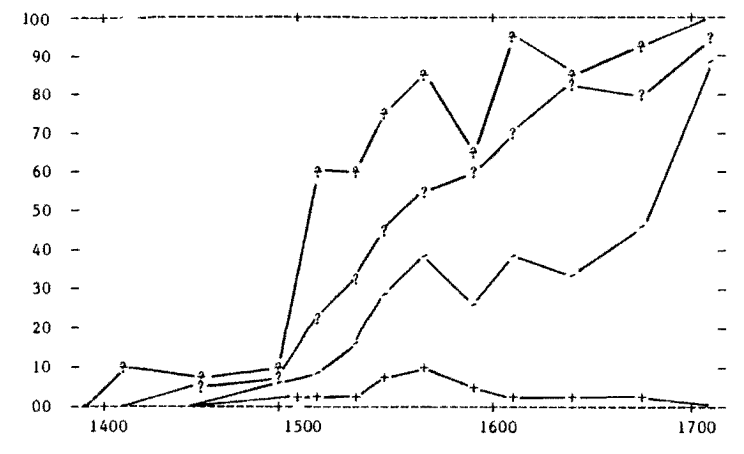
\includegraphics[width=.5\linewidth]{../images/kroch-graph}
		\caption{Frequency of do-support in different environments: affirmative and negative questions (? and \sout{?}) and affirmative and negative declaratives (+ and ') (Fig. 1 from \citealt{Kroch.1989})}
		\label{fig:kroch-graph}
	\end{figure}

	For English `to'-use, there are two changes to be considered (reflecting the rise of the To Grammar and the Allomorphy Grammar). In order to study these changes, I extracted all tokens from the Parsed Corpora of Historical English \citep{Kroch.2000,Taylor.2003,Kroch.2004,Taylor.2006,Kroch.2010} containing the following recipient introducing verbs (verbs that also introduce goals, e.g., SEND, were excluded): ALLOT, APPOINT, ASSIGN, AYEVEN, BEHIEGHT, BEQUEATH, BETAKE, DAELAN, FEED, GIVE, GRANT, LEND, OFFER, OWE, PAY, PROFFER, PROMISE, RESTORE, SELL, SELLAN, SERVE, SHOW, VOUCHSAFE, and YIELD. I also extracted information about whether the arguments were full noun phrases or pronouns, the relative order of the recipient and theme (and their order with respect to the verb to rule out cases of topicalisation), and whether or not the recipient was marked with `to' (passive data was also collected, which is discussed in the subsection below). 
	
	When the theme is a pronoun, the theme--recipient order was essentially categorical (31 examples of recipient--theme order over 1000 years out of INSERT HERE examples with theme pronouns). Since there was such poor evidence for the frequency of `to'-use in these environments, their inclusion muddled any attempts at statistical analysis. Therefore, those cases have been excluded for the analyses discussed below.

	In the theme--recipient order, the To Grammar and the Allomorphy Grammar generally produce the same forms. This is because the Allomorphy Grammar only produces a different surface form from the To Grammar when the recipient is adjacent to the verb. In all other cases, the two grammars produce identical surface forms. Since, in theme--recipient orders, the theme intervenes between the recipient and the verb (e.g., ``John gave the book to Mary''), this environment is generally unaffected by the incoming Allomorphy Grammar. The only exception to this is when the theme is a pronoun (as explained in Chapter \ref{ch:active}), since the theme pronoun can cliticise and thus cease to be an intervener.

	\begin{exe}
		\exr{ex:nw-brit-P} Northwestern British English:
		\begin{xlist}
		\ex[ ]{John [gave=it] [P=$\emptyset$ Mary]}
		\ex[*]{John [gave] [the book] [P=$\emptyset$ Mary]}
	\end{xlist}
	\end{exe}

	The aforementioned effects (i.e. the general lack of an effect of the Allomorphy Grammar and the exception when the theme is a pronoun) can be seen in the quantitation data. As can be seen in Figure \ref{fig:brit-tr}, all of the changes show the S-shaped curve that is the predicted outcome of logistic regression (as also seen in Figure \ref{fig:kroch-graph} for the do--support data). However, not all of the curves go to 100\%. When the theme is a pronoun, the curves level out below 100\% (reflecting the effect of theme cliticisation). The rate of `to' use in these contexts (when the theme is a pronoun) reflects the interaction of three properties: (a) the current rate of the To Grammar, (b) the current rate of the Allomorphy Grammar, and (c) the rate of theme cliticisation. Given that there is no independent way of finding the rate of theme cliticisation, these cases are also excluded from the quantitative analysis below.

	\begin{figure}[ht!]
		GENERATE FIGURE
		\caption{LOESS fits for theme--recipient data in different combinations of theme and recipient status (points indicate raw frequencies)}
		\label{fig:brit-tr}
	\end{figure}

	Focusing on the data where the theme is a full noun phrase, the effect of the Allomorphy Grammar is clearly seen in the recipient--theme order (without the interferring effect of theme cliticisation). In the recipient--theme order, there is direct competition between the To Grammar and the Allomorphy Grammar as to the realisation of P$_{dative}$ (either as `to' or as $\emptyset$). As can be seen in Figure \ref{fig:brit-tn}, the use of `to' initially rises in the recipient--theme order and then declines. I claim that this rise--fall pattern represents the initial rise from the adoption of the To Grammar, followed by a decline as the Allomorphy Grammar is adopted.

	\begin{figure}
		GENERATE FIGURE
		\caption{Model fits for data with full noun phrase theme (points indicate raw frequencies)}
		\label{fig:brit-tn}
	\end{figure}
	
	According to the causal explanation of the Constant Rate Effect (i.e., that the constant rate reflects the rate of adoption of a single underlying grammatical change), a Constant Rate Effect should hold between the rise portion of the recipient--theme data and the rise in the theme--recipient data, since both reflect the underlying adoption of the To Grammar. In order to test the Constant Rate Effect, however, it is necessary to disentagle the role of the To Grammar and the Allomorphy grammar in deriving the rise--fall pattern in the recipient--theme context. 

	The Subset Principle (formally implemented in Distributed Morphology, \citealt{Halle.1993}, but widely accepted in many morphological theories) states that the more specific of two forms competing for realisation of the same features is realised. A simple example is the case of irregular verbs, where the irregular rule (e.g., the past tense of `ring' is `rang') beats the more general regular rule (i.e., the past tense of a verb is formed by adding `ed', here leading to `ringed'). In this case, the Subset Principle states that if the Allomorphy Grammar is adopted, then for recipient--theme orders it does not matter whether the Null Grammar or the To Grammar is selected as the general default, the more specific null form will be inserted. However, if the Allomorphy Grammar is \textbf{not} selected, then the choice between the Null Grammar and the To Grammar decides which form gets realised. This can be captured with a 2x2 table reflecting whether the old or innovative form of being used for each change.

	\begin{table}
		\begin{tabular}{ccc}
					& No Allomorphy Grammar & Allomorphy Grammar\\
			Null Grammar	& John gave him the book & John gave him the book\\
			To Grammar	& John gave \textbf{to} him the book & John gave the book to him\\
		\end{tabular}
		\citation{2x2 table showing the recipient--theme realisation for the interaction between the two changes in dative P realisation in English}
		\label{tab:2x2int}
	\end{table}

	As can be seen in Table \ref{tab:2x2int}, the only way to get `to' in the recipient--theme context is to \textbf{adopt} the To Grammar and \textbf{not} adopt the Allomorphy Grammar. Given that our logistic regression is trying to predict the probability of `to', it is necessary to create a formula that derives the probability of `to' from the interaction of the probability of each change applying. The probability of `to' in the recipient--theme order is equal to the probability of \textbf{both} adopting the To Grammar and not adopting the Allomorphy Grammar. Probability theory states that the probability of two independent events both occuring is equal to the probability of the two events multiplied together. If $p$ represents the probability of adopting the To Grammar and $q$ represents the probability of adopting the Allomorphy Grammar, the probability of not adopting the Allomorphy Grammar is equal to $(1-q)$. Taken together, this means that the probability of `to' in the recipient--theme order is equal to $p * (1-q)$. Both p and q can be modelled with their own logistic function, which means that the Constant Rate Effect can be tested for in each change.\footnote{For details about how the model was fit, see Appendix A for a link to the relevant R files}

	A single model was fit that predicted both the theme--recipient and recipient--theme orders for data with full noun phrase themes using the equation applied above (modified so that q = 0 in the theme--recipient order, so only the p equation would apply). The full model contained effects for year, recipient type, and object order as well as their interaction. The optimal model was selected to have the lowest AIC.\footnote{AIC, Akide Information Critereon, is a way of selecting models that fit the data well, while taking into account the fact that adding more independent variables always improves fit. Comparing AIC, selects the model that finds an optimal balance between fitting well and having few independent variables.} 
	
	The optimal model had the following properties (model fits shown in Fig. \ref{fig:brit-tn}): (a) the first change was characterised by an intercept, an effect of year, an effect of word order and an effect of recipient status, (b) the second change was characterised by an intercept, an effect of year, and effect of recipient status, and an interaction between year and recipient status. The effects in model (a) indicate a Constant Rate Effect for the introduction of `to'-marking for recipients; there was no significant interaction between conditions. While `to'-marking raises at the same rate across all conditions, recipient--theme orders and recipient pronouns show less `to'-use in any given year. 
	
	As discussed above, failing to find a significant interaction is not enough to automatically claim that the Constant Rate Effect was found, it is possible that there was insufficient data to find a substantial violation of the Constant Rate effect. This explanation for the Constant Rate Effect finding in the first change (adoption of To Grammar) becomes less plausible, given that a significant interaction was identified for the second change (adoption of Allomorphy Grammar) indicating that there was enough power to identify interactions. The identification of a significant interaction for the second change strongly suggests that the Allomorphy Grammar actually reflects two different changes (one for recipient nouns and one for recipient pronouns). The effect of year was found to be higher for recipient pronouns, suggesting that the Allomorphy Grammar affected recipient pronouns faster than full noun phrases.
	
	Since many languages have a strong differentiation between recipient marking on full noun phrases and pronouns (e.g., Romance language differences between full noun phrases marked with \textit{a} `to' and clitic pronouns marked with synthetic case marking), this differentiation between full noun phrases and pronouns is not unexpected. It appears that there are actually two Allomorphy Grammars: one that applies to nouns, and another that applies to pronouns, which both have the same output, namely $\emptyset$, but which spread through the speech community at different rates. The grammar for pronouns rapidly spread through the speech community (possibly influenced by the fact that pronouns maintained some level of synthetic case marking), while the grammar for full noun phrases spread more slowly. This can be seen in Figure \ref{fig:brit-tn}, where the pronouns show a much less `to' use overall compared to full noun phrases.

	By modelling overlapping changes by multiplying thier independent probabilities, it was possible to confirm another case of the Constant Rate Effect. In this case, the Constant Rate Effect applied to the rise of the To Grammar. Given that there was independent support that the data was sufficient to detect meaningful interactions, there is solid evidence that the To Grammar was a unified change that applied during the Middle English period. As discussed in Chapter \ref{ch:active}, this supports the dative PP hypothesis by bolstering the notion that the `to' found in the modern theme--recipient orders is actually shared by the recipient--theme order. There was also usage evidence (supporting the judgement data from Northwestern British dialects) that theme cliticisation can license the null allomorph as part of the Allomorphy Grammar.
	
	Looking at the quantitative data also revealed another pronoun related feature of `to' use, namely that there are separate Allomorphy Grammars for full noun phrases and pronouns (i.e., recipient pronouns priveldge the null allomorph). Given that Romance clitic pronouns also show different morphological marking from their non-clitic counterparts, this distinction between full noun phrases and pronouns can be viewed as additional evidence for the existence of pronoun specific (i.e., clitic-like) effects in the grammar of Modern British English. Independent evidence about clitic-like effects for both recipients and pronouns increases the likelihood that the theme cliticisation explanation for sentences like (``John gave it him'') are on the right track.

\section{Passivisation}

	This section deals with quantitative data on passivisation with recipient ditransitives 

\subsection{Old English}
	The situation in Old English is quite complex. \cite{Allen.1999} provides evidence that monotransitive datives are able to become oblique subjects in Old English, but she suggests that in ditransitives, putative oblique subjects are actually topics. To discuss this distinciton, she introduces the term ``fronted dative'', which is agnostic as to whether the fronted element is a topic or a subject. The argument about the status of fronted datives in ditransitive passives is made on the basis of Coordinate Subject Deletion facts. In Old English (as in Modern English), arguments are generally obligatory (i.e., neither subject nor object drop is generally licensed). However, when two sentences are coordinated and share the same subject, the subject does not need to be expressed in the second sentence (\ref{ex:OECSD}). In a corpus investigation, none of the fronted datives in ditransitive passives triggered Coordinate Subject Deletion, while a number of fronted nominatives did (see Table \ref{tab:AllenOECSD}). 

	\begin{table}[t]
		\begin{tabular}{cccc}
			Nominative Coreferential & & Deletion & No Deletion \\
			& Order NOM DAT & 11 & 4 \\
			& Order DAT NOM & 4 & 3 \\
			& Total & 15 & 7 \\
			\hline
			Dative Coreferential & & Deletion & No Deletion \\
			& Order NOM DAT & 0 & 27 \\
			& Order DAT NOM & 0 & 11 \\
			& Total & 0 & 38 \\
		\end{tabular}
		\caption{Allen's counts of Coordinate Subject Deletion with ditransitive passive in OE prose (Table 2-6, \citealt{Allen.1999})}
		\label{tab:AllenOECSD}
	\end{table}

	\begin{exe}
		\ex \label{ex:OECSD} Old English:
		\gll and him comon \textbf{englas} to, and him ðenodon\\
		and him.DAT came \textbf{angels.NOM} to, and him.DAT served\\
		\trans ` and to him angels came and him (they) served \citep[ex. 34]{Allen.1999}.''
	\end{exe}

	The main problem with this conclusion is that there were only a small number of Old English coordinated examples, such that the lack of deletion for datives could be accidental. For the rest of this section, I do not take a stand on whether the arguments in Old English were subjects or not. I focus instead on general changes in word order (independently of whether that order is derived from subject raising or topicalisation). Before turning to changes in word order, changes in recipient marking need to be addressed.

	\subsection{Changes to Grammar}

	There are two changes going from Early Middle English to Modern American English that affect the grammar of recipient ditransitive passivisation. As discussed in the introduction to this chapter, a grammar distinguishes between strings that are associated with at least one meaning (grammatical strings) and strings that have no association with a meaning (ungrammatical strings). A change to the grammar, thus, means that some strings need to move from one category to another.\footnote{Another type of change in grammar would be a change in the association between meanings among grammatical strings. A grammatical string could be associated with a new meaning, or loose an association with an old meaning, while still being grammatical (i.e., still having some possible interpretations associated with it).} Concerning the passivisation of recipient ditransitives, the two changes are: (a) oblique recipient subjects vs. nominative recipient subjects and (b) availability of direct theme passivisation vs unavailability of direct theme passivisation. 

	As discussed in the previous subsection, it is unclear whether or not Old English had oblique subjects in the passives of recipient ditransitives. During the early Middle English period, it is difficult to tell whether fronted recipients are subjects (for the same reasons discussed concerning Old English in the previous subsection). Since synthetic case marking had been lost (for full noun phrases) by Early Middle English and since the To Grammar (see the previous section) was not yet universal (FIX WORDING), it is also difficult to determine whether a fronted recipient was nominative or dative. \cite{Allen.1999}, after carefully examining the extant Middle English corpus, identifies that the first unambiguous case of a nominative recipient subject in the passive of a ditransitive occurs in 1375. This reflects a change in the grammar of English, in so far as previously nominative recipient subjects were ungrammatical and now they are grammatical.

	Under the analysis described in Chapter \ref{ch:passive}, the nature of this grammar change reflects the availability of P-incorporation.Without P-incorporation, the only possible form of recipient passivisation is to have oblique subjects. Given that P-incorporation also generates pseudopassives, the simple prediction would be that pseudopassives would enter the language at the same time as nominative recipient passives. \cite{Sigursson.2014} showed that pseudopassivisation comes into the language in the beginning of the Middle English period. Indeed, as seen in Figure \ref{fig:recpas-pseudo}, pseudopassivisation and nominative recipient passivisation increase in use from about 1200 until 1650, when they both level off.

	\begin{figure}[ht!]
		INSERT FIGURE
		\caption{Loess curves showing rates of nominative recipient passivisation and pseudopassivisation in English}
		\label{fig:recpas-pseudo}
	\end{figure}

	Neither pseudopassivisation nor nominative recipient passivisation go to 100\%. For pseudopassivisation, this is expected. If the pseudopassivisation rate was 100\% that would mean that there were no active sentences with PP objects, which is highly improbable. For nominative recipient passivisation, it is less clear why the process should not go to completion, since this is the probability of having a nominative subject given that recipient passivisation has occurred, which could reasonably occur 100\% of the time. However, two residual cases prevent this from occurring. Looking at the examples of oblique recipients from the period after 1500, almost all of them are imperatives of the form ``To X, be this given/sent/delivered'', which seem to have been a common formula for deliveries. The other case is locative inversion, for which there is disagreement in the literature about the correct analysis. It seems likely that locative inversion is actually a type of topicalisation and not subject raising (CITATION), which means that these cases should actually be excluded (given that they are surface identical to subject raising with oblique dative subjects in these cases, it is impossible to exclude them automatically).

	This would seem to be a good case to look for a Constant Rate Effect (see the previous section). However, there are two problems that prevent looking for a constant rate effect. As can be seen in Figure \ref{fig:recpas-pseudo}, there is a great deal of uncertainty about the rise of nominative recipient passivisation, because there is very little data on recipient passivisation (see the next subsection for a discussion of why there is little data). Thus, even if a Constant Rate Effect was found (i.e., there was no significant interaction between year and pseudopassive vs nominative recipient passive), this could easily be attributed to the lack of data concerning recipient passives. Secondly, the fact that the changes do not go to 100\% means that standard techniques for fitting the logistic regressions cannot be used. Unfortunately, as of this time, I know of no methods for reliably fitting such models. In spite of not being able to quantitatively verify the existance of a Constant Rate Effect, the qualitative similarity in time course between the rise of pseudopassivisation and nominative recipient passivisation supports the notion that they are both derived via the same mechanism (namely P-incorporation).

	The second change in the grammar of ditransitive passivisation occurs within the history of American English. This change is the loss of direct theme passivisation, where the theme raises across the recipient to subject position (for more discussion see Chapter \ref{ch:passive}). In English, direct theme passivisation can be identified by the presence or absence of `to' before the recipient. If the theme scrambles to the left of the recipient before raising to subject position, then its lower copy intervenes between the recipient and the verb, preventing the null allomorph from being used. 
	
	Direct theme passivisation was argued to result from the locality properties of T in looking for a subject to move (i.e., is a PP in the search domain for subject movement). When direct theme passivisation is possible, PPs are invisible for subject movement. In the new grammar, however, they become defective interveners (i.e., they are not valid targets for the search, but they prevent the search from progressing further down the tree). The loss of direct theme passivisation can be operationalised as the replacement of T with the invisible search property with one with defective intervention. The trajectory of this change can be seen in Figure \ref{fig:loss-of-dt-in-amen}.

	\begin{figure}[ht!]
		INSERT FIGURE
		\caption{Loess curves showing the loss of direct theme passivisation with GIVE and OFFER in American English}
		\label{fig:loss-of-dt-in-amen}
	\end{figure}

	Connect to

	\subsection{Changes in Use of Grammar}

\section{Conclusions}
	In this chapter, I have presented two case studies of change in the history of English. The first captured changes in morphological marking of recipients, which supports the interchangeability of prepositional and synthetic case marking. The second the fall and rise of recipient passivisation. The first change provided an example of how even complex changes involving the interaction of a number of moving parts (two changes each of which involved scaling factors) can be broken apart using relatively simple statistical processes. The breaking apart of interacting changes provides evidence for the structure of the underlying grammar using the implications of the Constant Rate Effect. The second change provided some insight into the underlying mechanism driving changes in use frequency of syntactic mechanisms. In at least some cases, it is the surface outcome of the mechanisms that is subject to change (i.e., recipient passives), independently of how that surface property is derived (i.e., oblique subjects vs. dative-to-nominative raising). While in many cases the surface properties that drive use-frequency changes are the direct reflexes of grammatical properties (as was the case with changes in allomorphy in the `to'-marking change), in other cases the relationship between use and grammar is more indirect with surface properties that have multiple grammatical causes being unified by language learners.

\bibliography{diss}
